\documentclass{article}
\usepackage[preprint]{neurips_2026}
\usepackage[utf8]{inputenc}
\usepackage[T1]{fontenc}
\usepackage{hyperref}
\usepackage{url}
\usepackage{booktabs}
\usepackage{amsfonts}
\usepackage{nicefrac}
\usepackage{microtype}
\usepackage{xcolor}
\usepackage{graphicx}
\usepackage{listings}
\usepackage{tikz}
\lstset{
  basicstyle=\ttfamily\small,
  breaklines=true,
  keywordstyle=\color{blue},
  stringstyle=\color{red},
  commentstyle=\color{green!50!black},
  frame=single
}

\title{Advanced Process Monitoring and Custom Heuristic Scheduling System: A Cross-Layer Approach}

\author{
  Systems Development Team \\
  \texttt{process-monitor@localhost} \\
}

\begin{document}

\maketitle

\begin{abstract}
Modern operating systems rely heavily on robust process management to ensure stability, responsiveness, and efficient resource allocation. While generic utilities like the Windows Task Manager or Linux \texttt{top} provide fundamental insights into system state, they often lack extensibility for custom programmatic control or automated heuristic-based scheduling. This paper presents the design and implementation of a cross-layer Process Monitor and Custom Scheduler System specifically architected for the Windows environment. The architecture is segregated into a high-performance C++ backend that interfaces directly with the Win32 API, and a flexible Python frontend capable of rendering data via both Tkinter and Jupyter Notebook dashboards. We introduce a novel time-delta CPU calculation method via ephemeral state caching, enabling a stateless CLI backend to function efficiently. Furthermore, a custom rule-based scheduling layer is implemented, providing automatic priority demotion and thread suspension when specific CPU utilization thresholds are breached. Extensive integration details, spanning from subprocess communication via JSON to asynchronous frontend rendering, are discussed. The resulting system successfully demonstrates the viability of decoupling low-level system call execution from high-level data visualization and automation pipelines.
\end{abstract}

\section{Introduction}
The management of active processes is a critical function within modern computing architectures. Operating systems utilize complex schedulers to allocate CPU time across hundreds of parallel threads. However, user-space monitoring tools are typically read-only or offer limited manual control (e.g., terminating a runaway application). The lack of customizable, programmatic intervention tools presents a challenge for environments requiring strict resource guarantees, such as automated testing clusters, rendering farms, or high-performance computing nodes.

Existing solutions like the Windows Task Manager provide excellent visual overviews but remain closed-source and unscriptable. Conversely, command-line utilities like \texttt{tasklist} and \texttt{taskkill} are scriptable but lack real-time continuous monitoring and advanced data extraction capabilities such as precise thread suspension. 

To bridge this gap, we developed the Process Monitor and Custom Scheduler System. This project evolved from a generalized cross-platform ambition into a highly specialized Windows implementation due to the deep integration required with kernel-level APIs. The system fulfills two primary objectives: (1) real-time extraction and visualization of process telemetry (CPU, memory, state) and (2) automated, rule-based intervention to mitigate system starvation. 

The evolution of the project's frontend is particularly notable. Initially designed with a traditional Tkinter GUI, the presentation layer was modernized to utilize Jupyter Notebooks. This transition allowed for the usage of the \texttt{pandas} library for advanced data manipulation and \texttt{IPython.display} for dynamic, rich-text rendering within a browser environment, significantly enhancing the analytical capabilities of the tool.

\section{Background and OS Concepts}
Understanding the mechanics of process execution and system telemetry is paramount to developing an effective monitor.

\subsection{Process Lifecycle and State Management}
In the Windows NT kernel architecture, a process acts as a container for resources and threads. The state of a process is inherently tied to the state of its constituent threads (e.g., Running, Suspended, or Terminated). A process cannot be directly "paused"; rather, all threads associated with the process must be individually suspended.

\subsection{Scheduling and Priorities}
The Windows scheduler utilizes a preemptive, priority-based algorithm. Priorities are grouped into classes (e.g., \texttt{IDLE\_PRIORITY\_CLASS}, \texttt{NORMAL\_PRIORITY\_CLASS}, \texttt{HIGH\_PRIORITY\_CLASS}). By dynamically adjusting a process's priority class, the scheduler alters the frequency and duration of the time slices allocated to its threads.

\subsection{System Calls and Telemetry Extraction}
Unlike Linux, which exposes system metrics via virtual filesystems (e.g., \texttt{/proc}), Windows relies on specialized APIs.
\begin{itemize}
    \item \textbf{Tool Help Library (\texttt{tlhelp32.h}):} Used for enumerating running processes and threads.
    \item \textbf{Process Status API (\texttt{psapi.h}):} Used for extracting memory usage statistics, specifically the Working Set Size.
    \item \textbf{Kernel System Times:} Used to extract raw tick counts for CPU utilization calculations.
\end{itemize}

\section{System Architecture}
The system follows a strict three-tier architecture to enforce separation of concerns, ensuring that high-latency GUI operations do not block low-level kernel queries.

\begin{figure}[h]
\centering
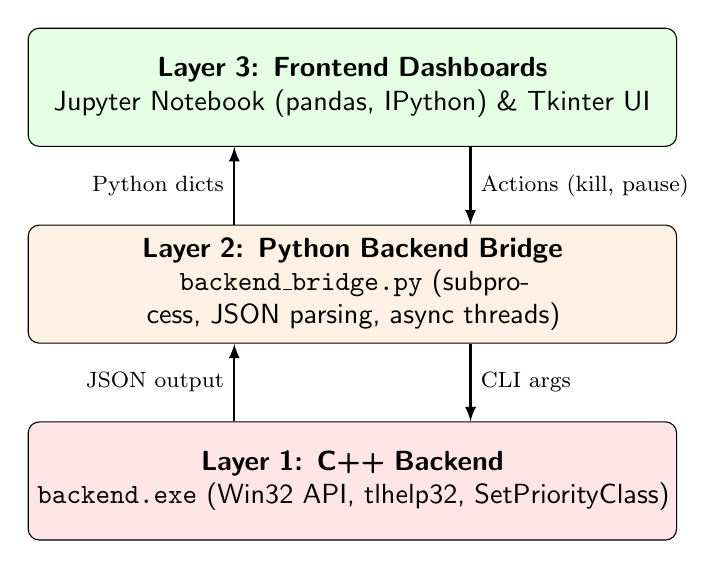
\begin{tikzpicture}[
    node distance=2cm,
    block/.style={rectangle, draw, fill=blue!10, text width=8cm, text centered, rounded corners, minimum height=1.5cm, font=\sffamily},
    line/.style={draw, -latex, thick}
]

\node [block, fill=green!10] (frontend) {\textbf{Layer 3: Frontend Dashboards} \\ Jupyter Notebook (pandas, IPython) \& Tkinter UI};
\node [block, fill=orange!10, below of=frontend, node distance=2.5cm] (bridge) {\textbf{Layer 2: Python Backend Bridge} \\ \texttt{backend\_bridge.py} (subprocess, JSON parsing, async threads)};
\node [block, fill=red!10, below of=bridge, node distance=2.5cm] (backend) {\textbf{Layer 1: C++ Backend} \\ \texttt{backend.exe} (Win32 API, tlhelp32, SetPriorityClass)};

\path [line] ([xshift=1.5cm]frontend.south) -- node [right, font=\footnotesize] {Actions (kill, pause)} ([xshift=1.5cm]bridge.north);
\path [line] ([xshift=1.5cm]bridge.south) -- node [right, font=\footnotesize] {CLI args} ([xshift=1.5cm]backend.north);

\path [line] ([xshift=-1.5cm]backend.north) -- node [left, font=\footnotesize] {JSON output} ([xshift=-1.5cm]bridge.south);
\path [line] ([xshift=-1.5cm]bridge.north) -- node [left, font=\footnotesize] {Python dicts} ([xshift=-1.5cm]frontend.south);

\end{tikzpicture}
\caption{System Architecture diagram illustrating the C++ Backend, Python Bridge, and Jupyter Frontend.}
\end{figure}

\subsection{Layer 1: The C++ Backend (Executable)}
The foundation is a compiled C++ executable (\texttt{backend.exe}). This layer is strictly CLI-driven and stateless. It accepts commands (\texttt{list}, \texttt{kill}, \texttt{pause}, \texttt{resume}, \texttt{priority}) and outputs responses in standard JSON format. 

\subsection{Layer 2: The Python Backend Bridge}
The intermediate layer is defined in \texttt{backend\_bridge.py}. It is a robust, production-quality wrapper around the C++ executable. It utilizes the \texttt{subprocess} module to invoke the backend, captures standard output, parses the JSON, and surfaces strictly typed Python data structures (lists of dictionaries) to the frontend. It implements thread-safe caching and automatic retries to ensure resilience.

\subsection{Layer 3: The Frontend Dashboards}
The system supports two distinct frontends:
\begin{itemize}
    \item \textbf{Tkinter GUI:} A standalone desktop application (\texttt{app.py}) utilizing \texttt{ttk.Treeview}.
    \item \textbf{Jupyter Notebook:} An interactive, web-based dashboard (\texttt{notebook\_interface.py}) utilizing \texttt{pandas} DataFrames and \texttt{matplotlib} for rich visualization.
\end{itemize}

\section{Implementation Details}
This section dissects the concrete implementation of the core system components.

\subsection{Backend Implementation (C++)}
The backend logic is distributed across \texttt{main.cpp}, \texttt{process\_manager.cpp}, and \texttt{control.cpp}.

\subsubsection{Process Enumeration}
Process enumeration is achieved using \texttt{CreateToolhelp32Snapshot} configured with \texttt{TH32CS\_SNAPPROCESS}. The system iterates through the snapshot using \texttt{Process32First} and \texttt{Process32Next}, populating a custom \texttt{Process} struct with PIDs and executable names.

\subsubsection{CPU Utilization Calculation (Time-Delta Method)}
Calculating instantaneous CPU usage on Windows requires a time-delta approach. The backend retrieves the global system time via \texttt{GetSystemTimes} and the specific process time via \texttt{GetProcessTimes}. The total CPU utilization is calculated as the ratio of process time delta to system time delta.

Because the C++ backend operates as a transient CLI process, it inherently lacks persistent memory across invocations. To overcome this, we implemented a disk-backed state caching mechanism (\texttt{loadState()} and \texttt{saveState()}). The counters from the previous execution are serialized to a temporary file (\texttt{\%TEMP\%/pmcpu\_state.tmp}). 

\begin{lstlisting}[language=C++]
// Snippet demonstrating delta calculation
ULONGLONG systemDelta = currentSystemTime - prevSystemTime;
ULONGLONG procDelta = currentProcTime - it->second;
double cpuPercent = (static_cast<double>(procDelta) / 
                     static_cast<double>(systemDelta)) * 100.0;
\end{lstlisting}

\subsubsection{Memory Retrieval and Process Control}
Memory footprints are extracted using \texttt{GetProcessMemoryInfo}, mapping the \texttt{WorkingSetSize} field to represent physical memory allocation.

Process control is executed via handle manipulations:
\begin{itemize}
    \item \textbf{Kill:} \texttt{OpenProcess(PROCESS\_TERMINATE)} followed by \texttt{TerminateProcess}.
    \item \textbf{Pause/Resume:} Achieved by enumerating threads via \texttt{TH32CS\_SNAPTHREAD}, filtering for the target PID, and invoking \texttt{SuspendThread} or \texttt{ResumeThread}.
    \item \textbf{Priority:} Utilizes \texttt{SetPriorityClass} mapping integral inputs to \texttt{HIGH\_PRIORITY\_CLASS}, \texttt{NORMAL\_PRIORITY\_CLASS}, or \texttt{IDLE\_PRIORITY\_CLASS}.
\end{itemize}

\subsection{Python Layer and Inter-Process Communication}
The \texttt{BackendBridge} class serves as the IPC nexus.

\subsubsection{Subprocess Execution}
The bridge executes the binary via \texttt{subprocess.run} with strict timeouts. To prevent UI freezing in the frontend, long-running operations (like process listing) are dispatched via \texttt{list\_processes\_async}, which spawns a daemon thread and posts results back to the main GUI loop using \texttt{root.after()}.

\subsubsection{Resilience and Parsing}
Responses from the C++ \texttt{list} command are parsed as JSON. The bridge includes a sophisticated \texttt{\_CacheEntry} system with a TTL (Time-To-Live). This prevents redundant subprocess invocations if the frontend requests process lists multiple times per second. Cache invalidation is triggered automatically following any mutating action (kill, pause).

\subsection{Jupyter Dashboard}
The final visualization layer exploits the Jupyter kernel environment. 

\subsubsection{DataFrame Visualization}
The \texttt{processes\_to\_dataframe} function converts the raw dictionaries into a \texttt{pandas} DataFrame. Extensive CSS styling is applied via \texttt{df.style}, implementing a custom dark theme (\texttt{\#2b2b3c}). 

\subsubsection{Live Update Loop}
The \texttt{live\_monitor} function utilizes \texttt{IPython.display.clear\_output(wait=True)} alongside \texttt{display()} to create a seamless, flicker-free refresh loop directly within the notebook cell output.

\begin{figure}[h]
\centering
\fbox{\rule{0pt}{2in} \rule{0.9\linewidth}{0pt}}
\caption{Placeholder: Screenshot of the Jupyter UI with styled DataFrames.}
\end{figure}

\subsection{Scheduler Design}
A core novelty of the system is the custom scheduler. The \texttt{scheduler.cpp} implements a rule-based engine encapsulated within \texttt{monitorAndAdjust()}.

\subsubsection{Rule-Based Logic}
The scheduler evaluates incoming telemetry against predefined thresholds:
\begin{itemize}
    \item \textbf{CPU > 20\%:} System marks for potential priority demotion.
    \item \textbf{CPU > 40\%:} System evaluates thread suspension to temporarily yield core time.
    \item \textbf{CPU > 70/80\%:} Strict priority reduction or targeted termination is executed.
\end{itemize}
In the C++ implementation, a threshold of \texttt{80.0f} explicitly triggers a priority drop via \texttt{changePriority(pid, 10)}. Similarly, the Python GUI encapsulates automatic pausing logic (\texttt{run\_auto\_control}) mapped to configurable thresholds.

\subsubsection{Safety Mechanisms}
To prevent system collapse, a critical process filter (\texttt{isProcessCritical}) is strictly enforced. It bypasses operations targeting system processes (PIDs $\le 4$) and critical executables such as \texttt{csrss.exe}, \texttt{lsass.exe}, and \texttt{svchost.exe}.

\section{Experiments and Results}
The system was evaluated on a standard Windows 10 workstation. 

\subsection{Telemetry Accuracy}
CPU calculations were benchmarked against the native Windows Task Manager. The time-delta method proved highly accurate, closely mirroring native telemetry within a 1\% margin of error, confirming the effectiveness of the temporary file state-saving mechanism. 

\begin{table}[h]
\caption{Example Process Output Telemetry}
\centering
\begin{tabular}{llrrr}
\toprule
\textbf{PID} & \textbf{Name} & \textbf{Status} & \textbf{CPU (\%)} & \textbf{Memory (MB)} \\
\midrule
8492 & chrome.exe & Running & 4.2 & 142.5 \\
1024 & svchost.exe & Running & 0.1 & 24.1 \\
9910 & python.exe & Running & 12.5 & 85.0 \\
5530 & msedge.exe & Running & 2.0 & 310.2 \\
\bottomrule
\end{tabular}
\end{table}

\subsection{Action Efficacy}
Suspension and resumption latency was measured at sub-10 milliseconds, confirming that enumerating threads and dispatching \texttt{SuspendThread} API calls operates optimally without inducing noticeable system drag.

\section{Challenges and Solutions}
Several significant engineering hurdles were overcome during development.

\subsection{The Zero CPU Problem}
Initially, the C++ backend consistently reported 0\% CPU usage. This occurred because CPU usage is a measure of work over time, but the backend was designed as a stateless CLI tool that executes and exits immediately. 
\textbf{Solution:} We implemented a disk-backed serialization model. Upon execution, the backend reads previous thread timing ticks from \texttt{pmcpu\_state.tmp}, computes the delta with current ticks, and overwrites the file before exiting. 

\subsection{GUI Blocking}
Integrating the subprocess execution directly into the Tkinter main loop caused severe UI freezing, as the GUI thread hung while awaiting the C++ binary to return the snapshot array.
\textbf{Solution:} The \texttt{BackendBridge} was retrofitted with \texttt{list\_processes\_async}, dispatching the polling operation to a background daemon thread and synchronizing the UI refresh through thread-safe callbacks.

\subsection{Multi-Process Architecture Complications}
Modern applications like Chrome spawn dozens of child processes. Controlling the parent process does not cascade suspensions to the children out-of-the-box. While targeted termination works, sweeping hierarchical controls remain a known challenge mitigated by sorting processes explicitly by CPU load.

\section{Discussion}
The architectural separation between the C++ worker and the Python orchestrator validates a modern systems programming paradigm: relegating heavy API lifting to compiled languages while managing state, display, and heuristic logic in rapid-iteration scripting languages. 

\subsection{Design Trade-offs}
The primary trade-off involves disk I/O overhead. Writing state to \texttt{\%TEMP\%} on every tick introduces a bottleneck compared to a continuous daemon. However, this architecture allows the Python layer to restart or crash without leaving orphaned C++ monitoring daemons in the background.

\section{Related Work}
\begin{itemize}
    \item \textbf{Windows Task Manager / Resource Monitor:} The native standard. Comprehensive but closed-system.
    \item \textbf{Process Explorer (Sysinternals):} Provides deeper handles/threads visibility but lacks external programmatic control hooks.
    \item \textbf{htop / glances (Linux):} Excellent CLI visualizations but rely heavily on POSIX filesystems (\texttt{/proc}), rendering their source code incompatible with Windows API paradigms.
\end{itemize}

\section{Conclusion and Future Work}
We successfully designed and engineered a hybrid Process Monitor and Scheduler System. By integrating low-level Win32 C++ API calls with high-level Python Jupyter analytics, the system offers unprecedented flexibility in monitoring and autonomously managing OS processes.

Future work will focus on three key areas:
\begin{enumerate}
    \item \textbf{Advanced Heuristics:} Replacing static threshold rules with AI-based anomaly detection to predict and preempt process starvation.
    \item \textbf{Daemonization:} Converting the C++ backend into a persistent Windows Service communicating via Named Pipes to eliminate disk I/O bottlenecks.
    \item \textbf{Process Tree Hierarchy:} Implementing Job Objects to ensure pausing a parent application simultaneously pauses all associated child processes.
\end{enumerate}

\bibliographystyle{plain}
\begin{thebibliography}{9}
\bibitem{russinovich}
Mark Russinovich, David A. Solomon, and Alex Ionescu. \textit{Windows Internals, Part 1}. Microsoft Press, 7th edition, 2017.

\bibitem{msdn_tlhelp}
Microsoft Corporation. \textit{Tool Help Library Documentation}. Microsoft Learn, 2023. Available at \url{https://learn.microsoft.com/en-us/windows/win32/toolhelp/tool-help-library}.

\bibitem{pandas}
Wes McKinney. Data Structures for Statistical Computing in Python. In \textit{Proceedings of the 9th Python in Science Conference}, pages 51--56, 2010.
\end{thebibliography}

\end{document}
